\documentclass[12pt]{article}

\fontfamily{lmss}
\usepackage{fullpage}
\usepackage{amsmath}
\usepackage{amsthm}
\usepackage{url}
\usepackage{multicol}
\usepackage{enumerate}
\usepackage{graphicx}
\usepackage{color}
\usepackage[labelfont=sc]{caption}
\usepackage{subcaption}
\usepackage[title]{appendix}
\usepackage{xcolor}
\usepackage{enumitem}
\usepackage{siunitx}

\usepackage{tikz}
\usetikzlibrary{graphs}
\usetikzlibrary{arrows.meta,shapes,shapes.geometric}
\usetikzlibrary{positioning, quotes}

\tikzset{
  % Two node styles for game trees: solid and hollow
  solid node/.style={circle,draw,inner sep=1.2,fill=black},
  hollow node/.style={circle,draw,inner sep=1.2},
  % styles for long branch labels
  left label/.style={above left,midway},
  right label/.style={above right,midway}
}

\usepackage{hyperref}
\hypersetup{
    colorlinks=true,
    linkcolor=blue,
    filecolor=magenta,      
    urlcolor=blue,
}

\usepackage{geometry}
\geometry{
  top=1in,            % <-- you want to adjust this
  bottom=1in,
  left=1in,
  right=1in,
  headheight=3ex,       % <-- and this
  headsep=4ex,          % <-- and this
}

\usepackage{lastpage}
\usepackage{fancyhdr}
\pagestyle{fancy}
\fancyhf{}
\renewcommand{\footrulewidth}{0.4pt}
\lhead{CS 486/686}
\rfoot{Page \thepage\ of \pageref{LastPage}}

\setlength{\parskip}{\baselineskip}%
\setlength{\parindent}{0pt}%

\usepackage{tcolorbox}
\tcbuselibrary{breakable}
\newenvironment{markscheme}
{
    \renewcommand{\parskip}{\baselineskip}
    \begin{tcolorbox}[
        colback=blue!10,
        colframe=blue!10,
        sharp corners,
        breakable
    ]
    \textbf{Marking Scheme:}
}
{
    \end{tcolorbox}
}

\newenvironment{sol}
{
    \renewcommand{\parskip}{\baselineskip}
    \begin{tcolorbox}[
        colback=magenta!10,
        colframe=magenta!10,
        sharp corners,
        breakable
    ]
    \textbf{Solutions:}
}
{
    \end{tcolorbox}
}

\newenvironment{example}
{
    \renewcommand{\parskip}{\baselineskip}
    \begin{tcolorbox}[
        colback=green!10,
        colframe=green!10,
        sharp corners,
        breakable
    ]
}
{
    \end{tcolorbox}
}

\lhead{CS 486/686}
\chead{Fall 2022}
\rhead{Assignment 3}
\cfoot{v1.0}
\lfoot{\copyright Blake VanBerlo 2022}

\title{CS 486/686 Assignment 3 \\ Fall 2022 \\ (125 marks) }
\author{Blake VanBerlo}
\date{Due Date: 11:59 pm ET on Tuesday, November 15, 2022}

\begin{document}

\maketitle

% \section*{Changes}

% \begin{itemize}

% \end{itemize}

\newpage

\newpage
\section*{Instructions}

\begin{itemize}
\item
Submit the signed academic integrity statement any written solutions in a file to the Q0 box in the A3 project on Crowdmark. \textbf{(5 marks)}.

\item Submit your written answers to questions 1 and 2 as PDF files to the Q1 and Q2 boxes respectively in the A3 project on Crowdmark. I strongly encourage you to complete your write-up in LaTeX, using this source file. If you do, in your submission, please replace the author with your name and student number. Please also remove the due date, the Instructions section, and the Learning Goals section. Thank you!

\item Submit any code to \verb+Marmoset+ at \url{https://marmoset.student.cs.uwaterloo.ca/}. Be sure to submit your code to the project named \texttt{Assignment 3 - Final}. 

\item
No late assignment will be accepted. This assignment is to be done individually.

\item
Lead TAs: 
\begin{itemize}
\item 
Connor Raymond Stewart (\url{crstewart@uwaterloo.ca})
\item
Dake Zhang (\url{dake.zhang@uwaterloo.ca})
\end{itemize}
The TAs' office hours will be scheduled and posted on LEARN and Piazza.
\end{itemize}



\section*{Learning goals}

{\bf Hidden Markov Models (HHM)}
\begin{itemize}
    \item Derive the formula for the prediction inference task in HMMs
    \item Trace the forward-backward algorithm
\end{itemize}

{\bf Decision Trees}
\begin{itemize}
\item 
Implement the decision tree learner algorithm to learn a decision tree using a dataset with real-valued features.
\item
Determine the accuracy of a decision tree on a dataset.
\item
Perform pre-pruning and post-pruning. Determine the best parameter value for pruning using $k$-fold cross validation.
\end{itemize}




\newpage
\section{Hidden Markov Models (30 marks)}
\label{question_hmm}

\begin{enumerate}[font=\Large,label=(\alph*)]

\item
In Lectures 10 and 11, we used a different form of the Bayes rule in our derivations for the filtering and smoothing formulas. Show that $P(A\,|\,B \land C) = \alpha P(B\,|\,A \land C) P(A\,|\,C)$, where $\alpha$ is a normalizing constant. In your derivation, clearly identify any probability rules that you use (see the rules in Lecture 6).

\begin{markscheme}

(2 marks) Correct derivation

(2 marks) Correct rules cited

\end{markscheme}

\item
Several commodities have been experiencing volatile prices recently, often due to supply chain issues and product shortages. Olive oil is an example of a product that might experience product shortages this year due to \href{https://www.cnn.com/interactive/2022/09/business/olive-oil-shortage-drought-cnnphotos/}{droughts in Europe}.

Suppose that you would like to determine the state of olive oil availability, given the price that you observe during your weekly grocery shopping trip. You model this problem as a Hidden Markov Model (HMM), where the hidden state $S_t$ is the state of olive oil supply (normal, supply chain backup, or shortage) and the observation is the price you see in the grocery store for a \SI{1}{L} bottle (low, normal, high). You make some assumptions regarding the transition and sensor distributions. For 3 weeks, you take note of the olive oil price, obtaining the HMM shown below:

\begin{center}
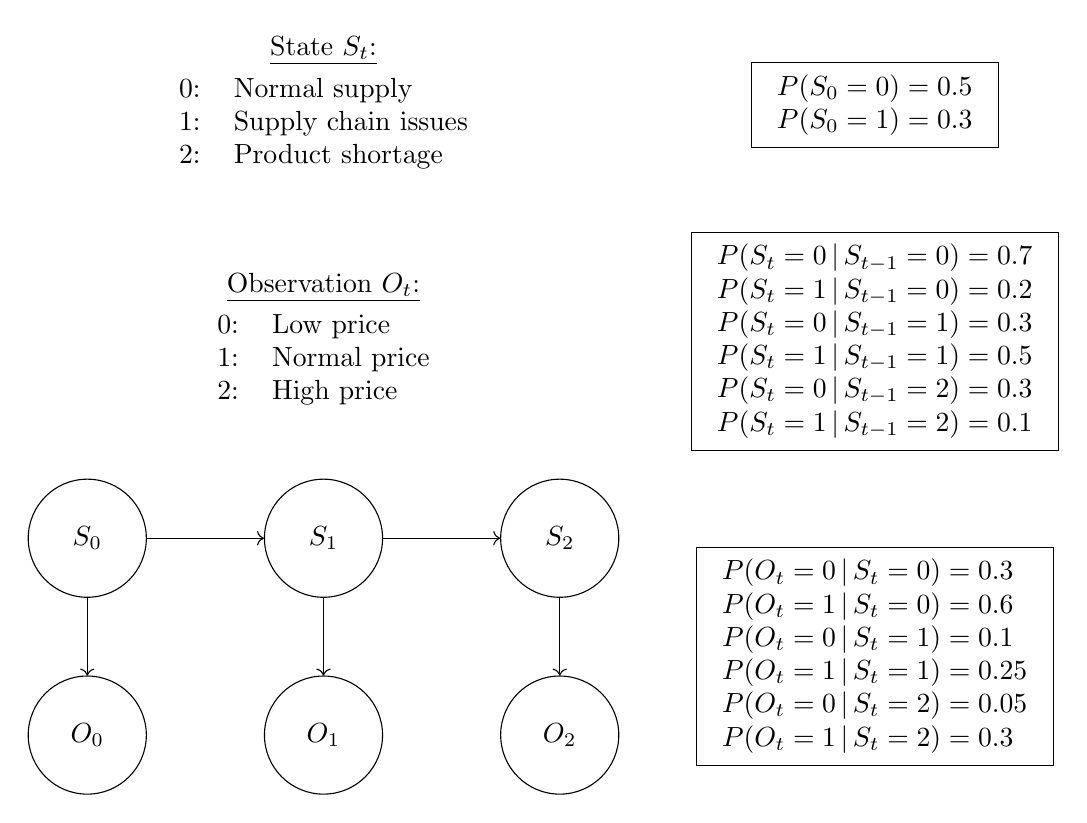
\begin{tikzpicture}[state/.style={circle, draw, minimum size=1.5cm}]

\node[draw] (tab1) at (10,10) {
\begin{tabular}{l}
$P(S_0=0) = 0.5$ \\
$P(S_0=1) = 0.3$ 
\end{tabular}
};

\node[draw] (tab2) at (10,7) {
\begin{tabular}{l}
$P(S_t=0 \,|\, S_{t-1}=0) = 0.7$ \\
$P(S_t=1 \,|\, S_{t-1}=0) = 0.2$ \\
$P(S_t=0 \,|\, S_{t-1}=1) = 0.3$ \\
$P(S_t=1 \,|\, S_{t-1}=1) = 0.5$ \\
$P(S_t=0 \,|\, S_{t-1}=2) = 0.3$ \\
$P(S_t=1 \,|\, S_{t-1}=2) = 0.1$ 
\end{tabular}
};

\node[draw] (tab3) at (10,3) {
\begin{tabular}{l}
$P(O_t=0 \,|\, S_t=0) =0.3$ \\
$P(O_t=1 \,|\, S_t=0) =0.6$ \\
$P(O_t=0 \,|\, S_t=1) =0.1$ \\
$P(O_t=1 \,|\, S_t=1) =0.25$ \\
$P(O_t=0 \,|\, S_t=2) =0.05$ \\
$P(O_t=1 \,|\, S_t=2) =0.3$ 
\end{tabular}
};

\node (rvs) at (3,10) {
\shortstack{ \underline{State $S_t$:} \\
\begin{tabular}{ll}
$0$: & Normal supply \\
$1$: & Supply chain issues \\
$2$: & Product shortage \\
\end{tabular}}
};

\node (rvs) at (3,7) {
\shortstack{ \underline{Observation $O_t$:} \\
\begin{tabular}{ll}
$0$: & Low price \\
$1$: & Normal price \\
$2$: & High price \\
\end{tabular}}
};

\node[state] (a) at (0, 4.5) {$S_0$};
\node[state] (b) at (3, 4.5) {$S_1$};
\node[state] (c) at (6, 4.5) {$S_2$};
\path[draw] [->] (a) -- (b);
\path[draw] [->] (b) -- (c);

\node[state] (e) at (0, 2) {$O_0$};
\node[state] (f) at (3, 2) {$O_1$};
\node[state] (g) at (6, 2) {$O_2$};
\path[draw] [->] (a) -- (e);
\path[draw] [->] (b) -- (f);
\path[draw] [->] (c) -- (g);

\end{tikzpicture}
\end{center}

You observed that the price of olive oil was normal in week $0$, high in week $1$, and high in week $2$. Execute the Forward Backward Algorithm to determine the probability distribution for the hidden state at each of weeks $0$, $1$, and $2$. That is, calculate $P(S_0 \,|\, O_0=1 \land O_1=2 \land O_2=2)$, $P(S_1 \,|\, O_0=1 \land O_1=2 \land O_2=2)$, and \\ $P(S_2 \,|\, O_0=1 \land O_1=2 \land O_2=2)$. Normalize each forward message. Show all calculations and round each calculation to $4$ decimal places. 

\begin{markscheme}

(10 marks) Correct execution of the Forward Backward Algorithm

(2 marks) \, Calculations are displayed clearly

\end{markscheme}

\item 
Recall that \textit{prediction} in Hidden Markov Models is the task of computing the probability distribution for the hidden state at some future time step. More specifically, prediction computes the distribution $P(S_k\,|\,o_{0:t})$, where $t$ is the current time step and $k$ is some future time step ($k > t$). 

Given the state distribution for time step $k \geq t$, show that the distribution for the state at time step $k + 1$ can be recursively computed as follows:

\begin{align*}
    P(S_{k+1}\,|\,o_{0:t}) = \sum_{s_k} P(S_{k+1}\,|\,s_k) P(s_k\,|\,o_{0:t})
\end{align*}

In your derivation, clearly identify any conditional independence assumptions and/or probability rules that you use.

\begin{markscheme}

(6 marks) Correct derivation

(2 marks) Correct rules/assumptions cited

\end{markscheme}

\item
After many time steps (i.e., the \textit{mixing time}), the distribution returned by prediction will converge to a fixed point. In other words, once convergence is reached, $P(S_{k}\,|\,o_{0:t})$ does not change as $k$ increases. This distribution is referred to as the \textit{stationary distribution} of the HMM.

What is the stationary distribution of the HMM in Question 1(b)? Show your calculations.

\begin{markscheme}

(4 marks) Correct answer and justification

(2 marks) Calculations are displayed clearly

\end{markscheme}


\end{enumerate}



\newpage
\section{Decision Trees (90 marks)}
\label{question_dt}

You will implement an algorithm to build a decision tree for the HTRU2 dataset. Read more about the dataset \href{https://archive.ics.uci.edu/ml/datasets/HTRU2}{here}.

{\bf Information on the provided code}

We have provided a dataset and four Python files. Please read the detailed comments in the provided files carefully.

\begin{table}[ht!]
    \centering
    \begin{tabular}{llp{11.9cm}}
         $1.$ & \verb+data.csv+ & Includes the dataset. {\bf Do not change this file.} \\[5pt]
         $2.$ & \verb+dt_global.py+ &  Defines several useful global variables {\bf Do not change the function signatures.} \\[5pt]
         $3.$ & \verb+dt_provided.py+ & Defines some useful functions for reading the dataset and splitting the dataset into different folds. Do not modify or submit this file. {\bf Do not change this file.} \\[5pt]
         $4.$ & \verb+dt_core.py+ & Contains empty functions for generating the tree and performing pruning. Include this file in your submission. {\bf Do not change the function signatures.} \\[5pt]
         $5.$ & \verb+dt_cv.py+ & Contains empty functions for performing cross validation. You need to complete all the empty functions in these files. {\bf Do not change the function signatures.} \\[5pt]
    \end{tabular}
    \label{tab:files_desc}
\end{table}

The dataset has real-valued features. When generating a decision tree, use {\bf a binary split} at each node. At each node in the decision tree, choose a feature and a split point for the feature using the procedure described on slide 48 of Lecture 13 to choose potential split points. The node should test whether a feature has a value greater than the split point or not. Along a path from the root node to a leaf node, we may test a real-valued feature multiple times with different split points.

{\bf The Attributes in an Anytree Node}

We use the \verb+anytree+ package to store the decision tree. Our unit tests make use of several custom attributes in an \href{https://anytree.readthedocs.io/en/latest/api/anytree.node.html#anytree.node.node.Node}{Anytree Node}. Make sure that you use these attributes so that you will pass our tests.

\begin{itemize}

\item \verb+name+: Each Node requires the \verb+name+ attribute, which is a string. The \verb+name+ of each node should be unique. You can generate this attribute in any way you like. We won't test this attribute.
% Otherwise, the plot of the tree will merge nodes that have the same \verb+name+s.

\item \verb+parent+: To construct the tree properly, you either need to set a Node's \verb+parent+ attribute (which is a Node as well) or a Node's \verb+children+ attributes. See \href{https://anytree.readthedocs.io/en/latest/api/anytree.node.html}{the Node documentation} for more details. We recommend setting the \verb+parent+ attribute of each Node. Once the \verb+parent+ attribute is set, the \verb+children+ attribute will be set automatically by Anytree. If you set the left child node's parent attribute before setting the right child node's parent attribute, then you can retrieve the left child node as \verb+children[0]+ and the right child node as \verb+children[1]+.

\item The \verb+feature+ attribute stores the chosen feature as a string. The \verb+split+ attribute stores the split point value as a float. Any non-leaf node should have the \verb+feature+ and \verb+split+ attributes.

\item The \verb+decision+ attribute stores the decision as an integer. Any leaf node should have the \verb+decision+ attribute.

\end{itemize}

{\bf Tie-Breaking Rules}

Please use the following tie-breaking rules to ensure that your program passes the unit tests.
\begin{enumerate}[1]
\item 
If a leaf node has examples with different labels, we need to determine a decision using majority vote. If there is a tie, return the label with the smallest value. For example, if a leaf node has two examples with label $4$ and two examples with label $5$, the majority decision should be $4$.

\item
Given a feature, if there are multiple split points with the same maximum information gain, choose the split point with the smallest value. For example, suppose that, the split points \verb+9.3+ and \verb+9.5+ tie for the maximum information gain among all the spilt points for the feature, we will choose to split on \verb+9.3+.

\item
Suppose that, for each feature, we have identified the split point with the maximum information gain. Given the best split points for the features, if multiple split points have the same maximum information gain, choose the first feature based on the order of the features in the first row of the \verb+data.csv+ file. 

For example, assume that feature $A$ comes before feature $B$ in the order. Suppose that the information gain for the best split point for $A$ and the best split point for $B$ tie for the maximum information gain (among the best split points for all the features), we will choose to split on the best split point for $A$.

\end{enumerate}

{\bf Floating Point Comparisons}

A correct implementation may fail the Marmoset tests due to floating point issues. To prevent this, please compare floating-point values using a tolerance. We have provided two functions \verb+less_than+ and \verb+less_than_or_equal_to+ in \verb+dt_provided.py+. Make sure that you use these functions when comparing floating-point values.

{\bf $k$-Fold Cross-Validation}

The purpose of performing cross validation is to choose the best value for a parameter. We will use $k$-fold cross validation with $k=10$ to choose the best parameter value in pre-pruning and post-pruning. 

In $10$-fold cross-validation, each data point serves double duty --- as training data and validation data. Below are the steps for conducting $10$-fold cross-validation.
\begin{enumerate}

\item 
Split the data into $10$ subsets using \verb+preprocess+ in \verb+dt_provided.py+.

\item 
For each parameter value, perform $10$ rounds of learning. In the $i$\textsuperscript{th} round, the validation set is the $i$\textsuperscript{th} fold and the training set consists of the remaining $9$ folds.

\item 
In the $i$\textsuperscript{th} round, learn a decision tree with the parameter value using the training set. Determine the prediction accuracy of the decision tree on the training set and on the validation set. The prediction accuracy is the fraction of examples that the tree predicts correctly. (Don't worry if you generate different trees in different rounds. We do not care about the trees generated. We only care about the prediction accuracies.)

\item 
After the $10$ rounds, calculate the average prediction accuracy of the decision tree on the training set and on the validation set, where the average is taken over the $10$ rounds. For each parameter value, you will produce two numbers: the average prediction accuracy on the training set and the average prediction accuracy on the validation set. 
 
\item 
Choose the parameter value with the highest average prediction accuracy on the validation set. 
\end{enumerate}

{\bf Packages: }

You can assume that numpy (version 1.19.5) and anytree (version 2.8.0) are available in our testing environment.

{\bf Efficiency: }

The unit tests will evaluate your implementation for correctness and efficiency. If your implementation does not terminate within a pre-defined time limit, it will fail the unit test. We set the time limits by taking our run-times and multiplying it by a small constant factor. For your information, our program terminates within \SI{5}{s} for part 2(b), \SI{160}{s} for part 2(c), and \SI{70}{s} for part 2(d).

Here is some advice for improving your program's efficiency. 
\begin{itemize}
\item Limit the external packages that your program uses. Do not use \verb+pandas+ --- it will slow down your program considerably. Limit your use of \verb+numpy+. It's sufficient to use Python arrays and dictionaries only.

\item Think of ways to perform pruning efficiently. You may be able to performing pruning without modifying the tree. You may also be able to start with a previously generated tree instead of building a full tree all over again.
\end{itemize}

{\bf Please complete the following tasks.}

\begin{enumerate}[font=\Large,label=(\alph*)]
\item 
Complete all the empty functions in \verb+dt_core.py+ and \verb+dt_cv.py+ and submit both files on Marmoset in a zipped folder.

\begin{markscheme}
(85 marks)

\begin{itemize}

% \verb+dt_core.py+

\item \verb+get_splits+ \\
(1 public test + 4 secret tests) * 2 marks = 10 marks

\item \verb+choose_feature_split+ \\
(1 public test + 4 secret tests) * 3 marks = 15 marks

\item \verb+split_examples+ \\
(1 public test + 4 secret tests) * 1 mark = 5 marks

\item \verb+learn_dt+ (and \verb+split_node+)

1 public test * 1 mark 
+ 2 simple secret tests * 2 marks 
+ 2 full-tree secret tests * 5 marks 
= 1 + 4 + 10 = 15 marks

\item \verb+predict+ \\
(1 public test + 4 secret tests) * 1 mark = 5 marks

\item \verb+get_prediction_accuracy+ \\
(1 public test + 4 secret tests) * 1 mark = 5 marks

\item \verb+post_prune+ \\
(1 public test + 4 secret tests) * 2 marks = 10 marks

% \verb+dt_cv.py+
\item \verb+cv_pre_prune+ \\
(1 public test + 4 secret tests) * 2 mark = 10 marks 

\item \verb+cv_post_prune+ \\
(1 public test + 4 secret tests) * 2 mark = 10 marks

\end{itemize}

\end{markscheme}

\item 
Suppose that we built a decision tree called \verb+tree-full+ using the dataset. What is the maximum depth of \verb+tree-full+? 

\begin{markscheme}

(1 mark) Correct value of the maximum depth of the tree.
\end{markscheme}

\item 
Suppose that we want to pre-prune \verb+tree-full+ using the maximum depth criterion and using majority voting to make decisions at leaf nodes. What is the best value of the tree's maximum depth through ten-fold cross-validation? Please use the range \verb+list(range(0, 40))+ for the maximum depth.

\begin{markscheme}

(1 mark) Correct value of the best maximum depth for pre-pruning.
\end{markscheme}

\item 
Suppose that we want to post-prune \verb+tree-full+ using the minimum expected information gain criterion.

For post-pruning, grow a full tree first. Define a value for the minimum expected information gain. Next, keep track of all the nodes that only has leaf nodes as its descendants. Let's call these nodes \verb+leaf parents+. For each \verb+leaf parent+ node, if the expected information gain is less than the pre-defined value, then delete its children and convert this node to a leaf node with majority decision. \verb+Repeat+ this process until the expected information gain at every \verb+leaf parent+ node is greater than or equal to the pre-defined value.

What is the best value for the minimum expected information gain through $10$-fold cross-validation? Use the range \verb+list(np.arange(0, 1.1, 0.1))+ for the minimum expected information gain.

\begin{markscheme}

(1 mark) Correct value of the best minimum expected information gain for post-pruning.
\end{markscheme}

\item 
In the previous parts, you have experimented with several ways of building a decision tree for the dataset. If you had a choice, what is the best strategy you can use to generate a decision tree for this dataset? You can choose one of the strategies in this assignment or you can think of any other strategies. 

Explain your strategy and justify why it is your best choice.
\begin{markscheme}

(2 marks) A reasonable explanation
\end{markscheme}

\end{enumerate}

\end{document}





























